\chapter{Numerical Principles and Error Analysis}
\label{ch:numerical-principles}

\section{Mathematical Framework: From Problems to Algorithms}
\label{sec:framework}

Before diving into error analysis, we must understand the fundamental structure of computational mathematics. Every numerical computation follows a pipeline from real-world phenomena to algorithmic solutions.

\subsection{Direct and Inverse Problems}
\label{subsec:direct-inverse}

At the heart of numerical mathematics lies the general problem:
\begin{equation}
    \boxed{F(x; d) = 0}
    \label{eq:general-problem}
\end{equation}
where:
\begin{itemize}
    \item $d$ represents the \emph{data} on which the solution depends
    \item $x$ is the \emph{solution} we seek
    \item $F$ models the \emph{relationship} between data and solution
\end{itemize}

\begin{example}{Linear Systems}{linear-system}
    For $F(x; b) = Ax - b = 0$, we solve the linear system $Ax = b$.
    Here $A$ is part of the model $F$, $b$ is the data, and $x$ is the unknown solution.
\end{example}

\paragraph{Classification of Problems}
\begin{description}
    \item[Direct Problem] Given $F$ and $d$, find $x$ such that $F(x; d) = 0$.
    \item[Inverse Problem] Given $F$ and $x$, determine the data $d$.
    \item[Identification Problem] Given $x$ and $d$, determine the model $F$.
\end{description}

\subsection{From Problems to Algorithms}
\label{subsec:algorithms}

\begin{definition}{Algorithm}{algorithm}
    An algorithm is a sequence of deterministic instructions consisting of elementary operations, designed to solve a problem and guaranteed to terminate in finitely many steps.
\end{definition}

We measure algorithms by three key criteria:
\begin{description}
    \item[Accuracy] How close do we get to the exact solution? How does error decrease as we invest more computational effort?
    \item[Reliability] How likely is it that the global error remains small? (Requires testing and statistical analysis)
    \item[Efficiency] What computational complexity is needed to achieve a desired accuracy?
\end{description}

\section{Well-Posedness: The Foundation of Stable Computation}
\label{sec:wellposed}

\begin{figure}[ht]
    \centering
    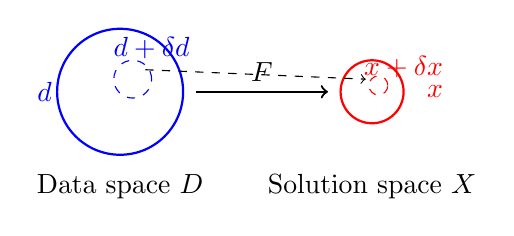
\begin{tikzpicture}[scale=0.8]
        % Well-posed problem illustration
        \draw[thick, blue] (0,0) circle (1);
        \draw[thick, red] (4,0) circle (0.5);
        \draw[->, thick] (1.2,0) -- (3.3,0) node[midway, above] {$F$};

        \node at (0,-1.5) {Data space $D$};
        \node at (4,-1.5) {Solution space $X$};

        % Small perturbation in data
        \draw[dashed, blue] (0.2,0.2) circle (0.3);
        \draw[dashed, red] (4.1,0.1) circle (0.15);
        \draw[->, dashed] (0.4,0.35) -- (3.9,0.2);

        \node[blue] at (-1.2,0) {$d$};
        \node[blue] at (0.5,0.7) {$d + \delta d$};
        \node[red] at (5,0) {$x$};
        \node[red] at (4.5,0.4) {$x + \delta x$};
    \end{tikzpicture}
    \caption{Well-posed problem: small changes in data $d$ lead to small changes in solution $x$.}
    \label{fig:wellposed}
\end{figure}

\begin{definition}{Well-Posedness (Hadamard)}{wellposed}
    The problem $F(x; d) = 0$ is \emph{well-posed} if:
    \begin{enumerate}
        \item \textbf{Existence:} A solution $x$ exists
        \item \textbf{Uniqueness:} The solution is unique
        \item \textbf{Continuous dependence:} The solution $x$ depends continuously on the data $d$
    \end{enumerate}
    If any condition fails, the problem is \emph{ill-posed} or \emph{unstable}.
\end{definition}

\subsection{Rigorous Definition of Continuous Dependence}
\label{subsec:continuous-dependence}

Let $D$ be the set of admissible data. Suppose we measure perturbed data $d + \delta d \in D$ instead of the true data $d \in D$. This yields a perturbed solution satisfying $F(x + \delta x; d + \delta d) = 0$.

\begin{definition}{Stability}{stability}
    A problem is \emph{stable} if there exist constants $\eta_0 = \eta_0(d) > 0$ and $K_0 = K_0(d)$ such that:
    \[
        \|\delta d\| \leq \eta_0 \quad \Rightarrow \quad \|\delta x\| \leq K_0 \|\delta d\|
    \]
\end{definition}

In words: small changes in data should yield proportionally small changes in the solution.

\section{Condition Numbers: Quantifying Sensitivity}
\label{sec:condition-numbers}

\subsection{Relative and Absolute Condition Numbers}
\label{subsec:condition-def}

\begin{definition}{Condition Numbers}{condition-numbers}
    For the problem $F(x; d) = 0$:

    \paragraph{Relative condition number:}
    \[
        \kappa(d) = \sup_{\substack{\delta d \neq 0 \\ d + \delta d \in D}} \frac{\|\delta x\|/\|x\|}{\|\delta d\|/\|d\|}
    \]

    \paragraph{Absolute condition number (when $d = 0$ or $x = 0$):}
    \[
        \kappa_{\text{abs}}(d) = \sup_{\substack{\delta d \neq 0 \\ d + \delta d \in D}} \frac{\|\delta x\|}{\|\delta d\|}
    \]
\end{definition}

\subsection{Computing Condition Numbers via Linearization}
\label{subsec:condition-computation}

Since $F(x; d) = 0$ has a unique solution, we can define the solution map $G: d \mapsto x$ implicitly via $F(G(d); d) = 0$.

For the error, $G(d + \delta d) = x + \delta x$. Assuming $G$ is differentiable with Jacobian $G'(d)$:
\[
    G(d + \delta d) = G(d) + G'(d)\delta d + o(\|\delta d\|) \quad \text{as } \delta d \to 0
\]

This gives us:
\[
    \boxed{
        \begin{aligned}
            \kappa(d)              & \approx \|G'(d)\| \frac{\|d\|}{\|G(d)\|} \\
            \kappa_{\text{abs}}(d) & \approx \|G'(d)\|
        \end{aligned}
    }
\]

\begin{example}{Square Root Problem - Ill-Conditioning}{sqrt-bad}
    Consider solving $x^2 - 2px + 1 = 0$ for $p \geq 1$. The solutions are $x_\pm = p \pm \sqrt{p^2 - 1}$.

    For the solution map $G_-(p) = p - \sqrt{p^2 - 1}$:
    \[
        G_-'(p) = 1 - \frac{p}{\sqrt{p^2 - 1}}
    \]

    The condition number becomes:
    \[
        \kappa(p) \approx \frac{|p|}{|p - \sqrt{p^2 - 1}|} \cdot \left|1 - \frac{p}{\sqrt{p^2 - 1}}\right| = \frac{p}{\sqrt{p^2 - 1}}
    \]

    For $p$ close to 1, $\kappa(p) \to \infty$ — the problem becomes ill-conditioned!
\end{example}

\begin{example}{Square Root Problem - Reformulation}{sqrt-good}
    Reformulate using $t = p + \sqrt{p^2 - 1}$, so $p = \frac{1 + t^2}{2t}$.

    The new problem: $F(x, t) = x^2 - \frac{x(1 + t^2)}{t} + 1 = 0$

    Solutions: $G_-(t) = t$ and $G_+(t) = \frac{1}{t}$

    Derivatives: $G_-'(t) = 1$ and $G_+'(t) = -\frac{1}{t^2}$

    Now $\kappa(t) \approx 1$ for any $t$ — much better conditioning!
\end{example}

\begin{remark}{Key Insight}{}
    A large condition number might indicate that you need to reformulate your problem, not just use higher precision arithmetic.
\end{remark}

\section{Why Worry About Error?}
\label{sec:why-error}

Imagine steering a ship with a compass that is \emph{almost} correct.
Each glance introduces a tiny angular mistake; over time these slips can
push the vessel far off course.
Numerical algorithms face the same danger: every arithmetic operation or
approximation injects a micro-error that may \emph{cancel}, \emph{accumulate},
or \emph{amplify}.

\emph{Error analysis} is the navigator's sea-chart. It answers:

\begin{itemize}
    \item where the error comes from (sources),
    \item how large it is now (bounds),
    \item how it propagates (stability),
    \item and how fast it shrinks as we refine the mesh or increase precision (convergence).
\end{itemize}

\section{Stability of Numerical Methods}
\label{sec:numerical-stability}

When we solve $F(x; d) = 0$ approximately through iterative methods, we work with sequences:
\[
    F_n(x_n; d_n) = 0, \quad n = 1, 2, \ldots
\]
where $x_n \to x$ and $d_n \to d$ as $n \to \infty$.

\begin{figure}[ht]
    \centering
    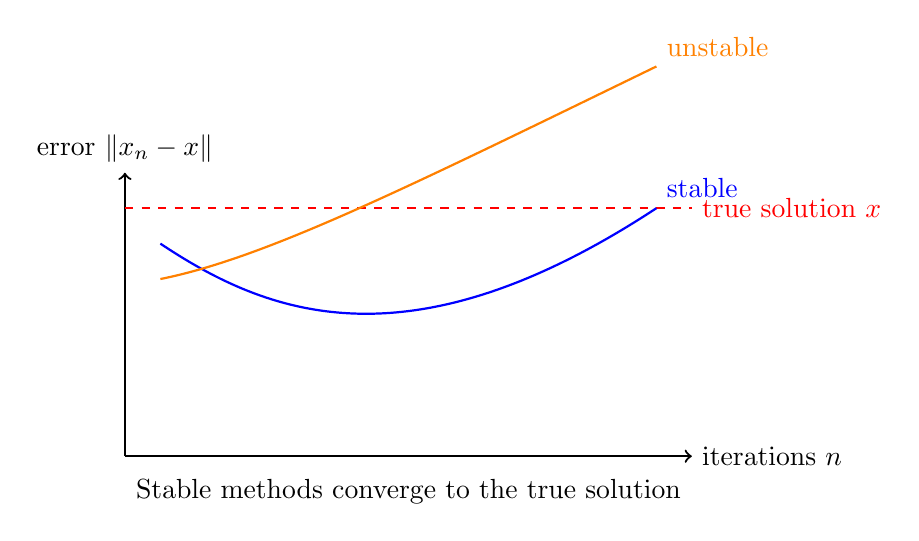
\begin{tikzpicture}[scale=0.9]
        % Convergence diagram
        \draw[->, thick] (0,0) -- (8,0) node[right] {iterations $n$};
        \draw[->, thick] (0,0) -- (0,4) node[above] {error $\|x_n - x\|$};

        % True solution line
        \draw[red, thick, dashed] (0,3.5) -- (8,3.5) node[right, red] {true solution $x$};

        % Stable convergence
        \draw[blue, thick] (0.5,3) .. controls (2,2) and (4,1.2) .. (7.5,3.5)
        node[above right, blue] {stable};

        % Unstable divergence
        \draw[orange, thick] (0.5,2.5) .. controls (2,2.8) and (4,3.8) .. (7.5,5.5)
        node[above right, orange] {unstable};

        \node at (4,-0.5) {Stable methods converge to the true solution};
    \end{tikzpicture}
    \caption{Stable vs. unstable numerical methods: error behavior over iterations.}
    \label{fig:stability}
\end{figure}

\subsection{Consistency, Stability, and Convergence}
\label{subsec:consistency}

\begin{definition}{Consistency}{consistency}
    A numerical method $F_n$ is \emph{consistent} with the continuous problem $F$ if:
    \[
        F_n(x; d) - F(x; d) \to 0 \quad \text{as } n \to \infty
    \]
    for any admissible data $d \in D$ and its exact solution $x$.
\end{definition}

\begin{definition}{Convergence}{convergence}
    A numerical method is \emph{convergent} if for all $\varepsilon > 0$, there exist $n_0 = n_0(\varepsilon)$ and $\delta = \delta(n_0, \varepsilon)$ such that:
    \[
        n > n_0 \text{ and } \|\delta d_n\| \leq \delta \quad \Rightarrow \quad \|x(d) - x_n(d + \delta d_n)\| \leq \varepsilon
    \]
\end{definition}
\begin{theorem}{Lax-Richtmyer Equivalence}{lax-richtmyer}
    For well-posed linear problems, a consistent finite difference method is convergent if and only if it is stable.
\end{theorem}

This fundamental theorem establishes the theoretical foundation for numerical analysis:

\[
    \boxed{\text{Consistency} + \text{Stability} \iff \text{Convergence}}
\]

\paragraph{Interpretation}
\begin{itemize}
    \item \textbf{Consistency} ensures each step approximates the differential equation correctly
    \item \textbf{Stability} prevents local errors from amplifying catastrophically
    \item \textbf{Convergence} guarantees the numerical solution approaches the exact solution as the mesh is refined
\end{itemize}

The theorem reveals that consistency alone is insufficient—without stability, small local truncation errors can grow exponentially, destroying convergence regardless of the method's formal order of accuracy.

\begin{example}{Third-Order Adams-Bashforth}{ab3step}
    Coefficients:
    \[
        \beta_0=\frac{5}{12},\quad
        \beta_1=-\frac{4}{3},\quad
        \beta_2=\frac{23}{12}
    \]
    give:
    \[
        u_{n+3}=u_{n+2}
        +h\left(\frac{23}{12}f_{n+2}-\frac{4}{3}f_{n+1}+\frac{5}{12}f_{n}\right)
    \]

    \paragraph{Local error}
    A fourth-order Taylor expansion yields:
    \[
        \tau_{n+3} = \frac{3}{8}h^{4}y^{(4)}(\xi_n) = \mathcal{O}(h^{4}),
    \]
    so the method is consistent with order $p=3$.
    \paragraph{Zero-stability}
    $\rho(r)=r^3-r^2=r^2(r-1)$ has roots $0,0,1$; all lie inside or on the unit circle and the unit root is simple.

    \paragraph{Convergence}
    By Dahlquist's theorem (the ODE analogue of Lax-Richtmyer):
    \[
        \max_{0\le n\le T/h}|u_n-y(t_n)|=\mathcal{O}(h^{3})
    \]
\end{example}


\subsection{A Priori vs. A Posteriori Error Analysis}
\label{subsec:error-analysis-types}

\begin{description}
    \item[A Priori Analysis] Estimates error bounds \emph{before} computation:
          \begin{itemize}
              \item \textbf{Forward Analysis:} Bounds $\|\delta x_n\|$ due to $\|\delta d\|$ or method properties
              \item \textbf{Backward Analysis:} Given computed $\hat{x}_n$, find $\delta d$ such that $F_n(\hat{x}_n; d + \delta d) = 0$
          \end{itemize}

    \item[A Posteriori Analysis] Estimates actual error using computed results:
          \begin{itemize}
              \item Estimate $\|\hat{x}_n - x\|$ using residual $r_n = F(\hat{x}_n; d)$
              \item Adaptive methods use this for step size control
          \end{itemize}
\end{description}

\section{Sources of Error}
\label{sec:sources}

Understanding error sources is crucial for developing reliable numerical methods. Errors propagate through a computational pipeline from the real world to our final answer.

\begin{figure}[ht]
    \centering
    \begin{tikzpicture}[node distance=2cm and 3cm, on grid, auto]
        \node[draw, rectangle, fill=blue!20] (real) {Real World Problem};
        \node[draw, rectangle, fill=green!20, right=of real] (math) {Mathematical Model $F$};
        \node[draw, rectangle, fill=yellow!20, right=of math] (discrete) {Discrete Method $F_n$};
        \node[draw, rectangle, fill=red!20, right=of discrete] (computed) {Computed Solution $\hat{x}_n$};

        \draw[->, thick] (real) -- (math) node[midway, above] {modeling};
        \draw[->, thick] (math) -- (discrete) node[midway, above] {discretization};
        \draw[->, thick] (discrete) -- (computed) node[midway, above] {round-off};

        \node[below=0.5cm of real] {$x_{\text{phys}}$};
        \node[below=0.5cm of math] {$x$};
        \node[below=0.5cm of discrete] {$x_n$};
        \node[below=0.5cm of computed] {$\hat{x}_n$};
    \end{tikzpicture}
    \caption{Error propagation pipeline: from physics to computation.}
    \label{fig:error-pipeline}
\end{figure}

The total error decomposes as:
\[
    \boxed{e_{\text{total}} = \underbrace{(x_{\text{phys}} - x)}_{\text{modeling}} + \underbrace{(x - x_n)}_{\text{discretization}} + \underbrace{(x_n - \hat{x}_n)}_{\text{round-off}}}
\]

\subsection{Modeling Error}
\label{subsec:modeling-error}

The mismatch between the \emph{mathematical model} and reality (e.g., replacing the Navier-Stokes equations by potential flow). No amount of numerical refinement can undo this bias.

\begin{example}{Modeling Error}{modeling-error}
    Using the linear heat equation $u_t = \alpha u_{xx}$ to model heat conduction neglects:
    \begin{itemize}
        \item Nonlinear temperature-dependent conductivity
        \item Radiation heat transfer
        \item Convective effects
    \end{itemize}
\end{example}

\subsection{Data Error}
\label{subsec:data-error}

Inexact initial or boundary data, coefficients, or forcing terms. For linear multistep ODE solvers these perturbations behave like round-off: they are injected at start-up and spread according to the method's stability.

\subsection{Discretization (Truncation) Error}
\label{subsec:discretization-error}

Approximating an infinite object by a finite stencil/series. A forward difference illustrates the idea:
\[
    f'(x) - \frac{f(x+h)-f(x)}{h} = \tfrac{h}{2}f''(\xi) = \mathcal{O}(h)
\]

The residual that remains after \emph{one} step is called the \emph{local truncation error (LTE)}.

\begin{figure}[ht]
    \centering
    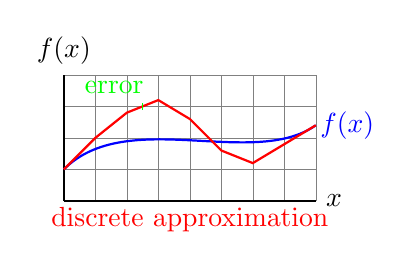
\begin{tikzpicture}[scale=0.8]
        % Grid showing discretization
        \draw[step=0.5cm, gray, very thin] (0,0) grid (4,2);
        \draw[thick] (0,0) -- (4,0) node[right] {$x$};
        \draw[thick] (0,0) -- (0,2) node[above] {$f(x)$};

        % Smooth function
        \draw[blue, thick] (0,0.5) .. controls (1,1.5) and (3,0.5) .. (4,1.2);
        \node[blue] at (4.5,1.2) {$f(x)$};

        % Discrete approximation
        \draw[red, thick] (0,0.5) -- (0.5,1) -- (1,1.4) -- (1.5,1.6) -- (2,1.3) -- (2.5,0.8) -- (3,0.6) -- (3.5,0.9) -- (4,1.2);
        \node[red] at (2,-0.3) {discrete approximation};

        % Error indication
        \draw[dashed, green] (1.25,1.55) -- (1.25,1.45);
        \node[green] at (0.8,1.8) {error};
    \end{tikzpicture}
    \caption{Discretization error: approximating a smooth function on a finite grid.}
    \label{fig:discretization}
\end{figure}

\subsection{Floating-Point (Round-Off) Error}
\label{subsec:roundoff-error}

Computers represent reals as:
\[
    x = \pm m \times 2^{e}, \qquad m,e\in\mathbb{Z}
\]
so most numbers are stored only approximately.

For every $\circ\in\{+,-,\times,/\}$:
\[
    \mathrm{fl}(x\circ y) = (x\circ y)\,(1+\delta), \qquad |\delta|\le\varepsilon_{\text{mach}}
\]

The \emph{machine epsilon} is the smallest $\varepsilon_{\text{mach}}$ with $1+\varepsilon_{\text{mach}}>1$; for IEEE double precision $\varepsilon_{\text{mach}}=2^{-53}\approx1.1\times10^{-16}$.

\begin{remark}{Catastrophic Cancellation}{}
    When subtracting nearly equal numbers, relative error can explode:
    \[
        \frac{(a + \delta a) - (b + \delta b)}{a - b} = 1 + \frac{\delta a - \delta b}{a - b}
    \]
    If $a \approx b$, then $\frac{\delta a - \delta b}{a - b}$ can be huge!
\end{remark}

\section{Measuring Error}
\label{sec:measuring-error}

\subsection{Local Truncation Error (LTE)}
\label{subsec:lte}

For a $k$-step multistep method:
\[
    \sum_{j=0}^k\alpha_j u_{n+j} = h\sum_{j=0}^k\beta_j f_{n+j}
\]

Insert the \emph{exact} solution $y$:
\[
    \tau_{n+k} = \frac{1}{h}\Bigl( \sum_{j=0}^{k}\alpha_j y(t_{n+j}) - h\sum_{j=0}^{k}\beta_j f(t_{n+j},y(t_{n+j})) \Bigr)
\]

If $\tau_{n+k}=\mathcal{O}(h^{p+1})$, the method has \emph{order $p$}.

\begin{figure}[ht]
    \centering
    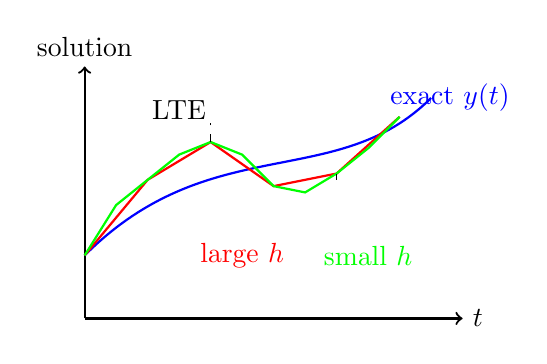
\begin{tikzpicture}[scale=0.8]
        % Step size comparison
        \draw[->, thick] (0,0) -- (6,0) node[right] {$t$};
        \draw[->, thick] (0,0) -- (0,4) node[above] {solution};

        % Exact solution
        \draw[blue, thick] (0,1) .. controls (2,3) and (4,2) .. (5.5,3.5);
        \node[blue] at (5.8,3.5) {exact $y(t)$};

        % Large steps
        \draw[red, thick] (0,1) -- (1,2.2) -- (2,2.8) -- (3,2.1) -- (4,2.3) -- (5,3.2);
        \node[red] at (2.5,1) {large $h$};

        % Small steps
        \draw[green, thick] (0,1) -- (0.5,1.8) -- (1,2.2) -- (1.5,2.6) -- (2,2.8) -- (2.5,2.6) -- (3,2.1) -- (3.5,2.0) -- (4,2.3) -- (4.5,2.7) -- (5,3.2);
        \node[green] at (4.5,1) {small $h$};

        % Error indication
        \draw[dashed] (2,2.8) -- (2,3.1);
        \draw[dashed] (4,2.3) -- (4,2.2);
        \node at (1.5,3.3) {LTE};
    \end{tikzpicture}
    \caption{Local truncation error decreases as step size $h$ becomes smaller.}
    \label{fig:lte}
\end{figure}

\subsection{Global Discretization Error (GDE)}
\label{subsec:gde}

After many steps:
\[
    e_n = u_n - y(t_n), \qquad n=0,1,\dots,N
\]

Under zero-stability:
\[
    \max_{0\le n\le N}|e_n| \;\le\; C\max_{0\le n\le N}|\tau_n|
\]

Thus for multistep methods, global and local orders coincide; for Runge-Kutta, global order is one lower than local order.

\section{Stability Types in Numerical Methods}
\label{sec:stability-types}

\subsection{Zero-Stability}
\label{subsec:zero-stability}

\emph{Zero-stability} is fundamental for \emph{linear multistep methods}. Unlike one-step methods, multistep methods use several past values, so errors can persist through the recurrence relation.

For a $k$-step method with characteristic polynomial $\rho(r)=\sum_{j=0}^k\alpha_jr^j$, zero-stability requires:
\begin{itemize}
    \item All roots satisfy $|r|\le1$
    \item Any roots on the unit circle are simple:
    \begin{align*}
        \rho(r) &= 0 \quad \text{for } |r|=1 \\
        \rho'(r) &\neq 0 \quad \text{for } |r|=1
    \end{align*}
\end{itemize}

\begin{figure}[ht]
    \centering
    \begin{tikzpicture}
        % Unit circle
        \draw[thick] (0,0) circle (2);
        \draw[->, thick] (-2.5,0) -- (2.5,0) node[right] {$\Re$};
        \draw[->, thick] (0,-2.5) -- (0,2.5) node[right] {$\Im$};

        % Zero-stable roots
        \filldraw[thm-color] (2,0) circle (0.1) node[below right] {stable: $|r| \leq 1$};
        \filldraw[thm-color] (1,1) circle (0.1);
        \filldraw[thm-color] (1,-1) circle (0.1);
        \filldraw[thm-color] (-0.5,0.8) circle (0.1);
        \filldraw[thm-color] (-0.5,-0.8) circle (0.1);

        % Unstable root
        \filldraw[red] (2.3,0.5) circle (0.1) node[above right] {unstable: $|r| > 1$};

        \node at (0,-3) {Zero-stable: all roots inside or on unit circle};
    \end{tikzpicture}
    \caption{Root condition for zero-stability of multistep methods.}
    \label{fig:zero-stability}
\end{figure}

\subsection{\texorpdfstring{$A$}{A}-Stability and \texorpdfstring{$L$}{L}-Stability}
\label{subsec:a-l-stability}

Let $\Phi(z)$ be the stability function for $y'=\lambda y$.

\begin{definition}{$A$-Stability and $L$-Stability}{}
    A method is:
    \begin{itemize}
        \item \textbf{$A$-stable} if $|\Phi(z)|\le1$ whenever $\Re z<0$
        \item \textbf{$L$-stable} if, in addition, $\Phi(z)\to0$ as $z\to-\infty$
    \end{itemize}
\end{definition}

\begin{figure}[ht]
    \centering
    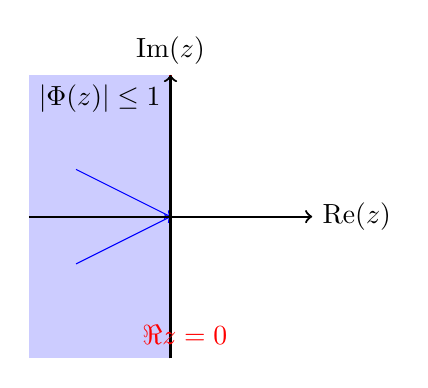
\begin{tikzpicture}[scale=0.6]

        % Left half-plane (stability region)
        \fill[blue!20] (-3,-3) rectangle (0,3);
        \node at (-1.5,2.5) {$|\Phi(z)| \leq 1$};

        % Stability boundary
        \draw[thick, red] (0,-3) -- (0,3);

        % Sample trajectories
        \draw[->, blue] (-2,1) .. controls (-1,0.5) .. (0,0);
        \draw[->, blue] (-2,-1) .. controls (-1,-0.5) .. (0,0);

        % Complex plane
        \draw[->, thick] (-3,0) -- (3,0) node[right] {Re($z$)};
        \draw[->, thick] (0,-3) -- (0,3) node[above] {Im($z$)};

        \node[red] at (0.3,-2.5) {$\Re z = 0$};
    \end{tikzpicture}
    \caption{$A$-stability region: the entire left half-plane.}
    \label{fig:a-stability}
\end{figure}

\subsection{Comparison of Stability Types}
\label{subsec:stability-comparison}

\begin{center}
    \begin{tabular}{@{}l l c c@{}}
        \toprule
        \textbf{Stability} & \textbf{Methods}    & \textbf{Stiffness-safe} & \textbf{Fast-mode damping} \\
        \midrule
        Zero-stable        & Multistep           & No                      & No                         \\
        $A$-stable         & One-step, Multistep & Yes                     & No                         \\
        $L$-stable         & One-step, Multistep & Yes                     & Yes                        \\
        \bottomrule
    \end{tabular}
\end{center}

\paragraph{Which to use?}
\begin{itemize}
    \item \textbf{Non-stiff:} Zero-stable multistep is sufficient
    \item \textbf{Stiff:} Choose an $A$-stable method for larger, stable steps
    \item \textbf{Very stiff:} Use an $L$-stable scheme for rapid damping of stiff modes
\end{itemize}

\section{Advanced Topics in Error Analysis}
\label{sec:advanced-topics}

\subsection{Conditioning vs. Stability}
\label{subsec:conditioning-vs-stability}

It's crucial to distinguish between:
\begin{description}
    \item[Well-conditioned problem] The mathematical problem $F(x; d) = 0$ has a small condition number
    \item[Stable algorithm] The numerical method produces solutions that are insensitive to perturbations
\end{description}

\begin{figure}[ht]
    \centering
    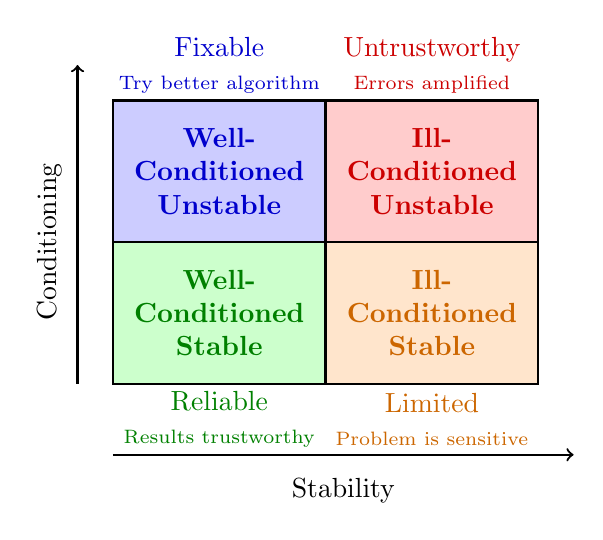
\begin{tikzpicture}[scale=0.9]
        % Color backgrounds (use more distinct colors)
        \fill[green!20] (0,0) rectangle (3,2);    % Well-conditioned, Stable
        \fill[orange!20] (3,0) rectangle (6,2);   % Ill-conditioned, Stable
        \fill[blue!20] (0,2) rectangle (3,4);     % Well-conditioned, Unstable
        \fill[red!20] (3,2) rectangle (6,4);      % Ill-conditioned, Unstable

        % Draw grid
        \draw[thick] (0,0) rectangle (3,2);
        \draw[thick] (3,0) rectangle (6,2);
        \draw[thick] (0,2) rectangle (3,4);
        \draw[thick] (3,2) rectangle (6,4);

        % Cell labels (larger, colored text)
        \node[align=center, text=green!50!black] at (1.5,1) {\textbf{Well-}\\\textbf{Conditioned}\\\textbf{Stable}};
        \node[align=center, text=orange!80!black] at (4.5,1) {\textbf{Ill-}\\\textbf{Conditioned}\\\textbf{Stable}};
        \node[align=center, text=blue!80!black] at (1.5,3) {\textbf{Well-}\\\textbf{Conditioned}\\\textbf{Unstable}};
        \node[align=center, text=red!80!black] at (4.5,3) {\textbf{Ill-}\\\textbf{Conditioned}\\\textbf{Unstable}};

        % Outcome labels (smaller, colored text)
        \node[align=center, text=green!50!black] at (1.5,-0.5) {Reliable\\\scriptsize Results trustworthy};
        \node[align=center, text=orange!80!black] at (4.5,-0.5) {Limited\\\scriptsize Problem is sensitive};
        \node[align=center, text=blue!80!black] at (1.5,4.5) {Fixable\\\scriptsize Try better algorithm};
        \node[align=center, text=red!80!black] at (4.5,4.5) {Untrustworthy\\\scriptsize Errors amplified};

        % Axes
    % Simple axes with labels
    \draw[->, thick] (-0.5,0) -- (-0.5,4.5);
    \node[rotate=90] at (-0.9,2) {Conditioning};

    \draw[->, thick] (0,-1) -- (6.5,-1);
    \node at (3.25,-1.5) {Stability};
    \end{tikzpicture}
    \caption{Conditioning (problem sensitivity) vs.\ stability (algorithm robustness): Only the lower-left is truly reliable. If the algorithm is unstable, try a better method; if the problem is ill-conditioned, no algorithm can fully fix it.}
    \label{fig:conditioning-stability}
\end{figure}

An ill-conditioned \emph{problem} means even the best algorithm will struggle; an unstable \emph{algorithm} can often be improved (e.g., by using pivoting or a more robust method).

\subsection{Backward Error}
\label{sec:backward}

Instead of asking "How wrong is my solution?" ask "Which \emph{nearby} problem did I solve \emph{exactly}?"

A $p$-th order Runge-Kutta method solves:
\[
    y' = f(t,y) + h^{p}g_h(t,y), \qquad g_h=\mathcal{O}(1)
\]
Long-time behavior (e.g., energy conservation in symplectic integrators) is often easier to explain in this \emph{modified equation} picture.
\begin{figure}[ht!]
    \centering
    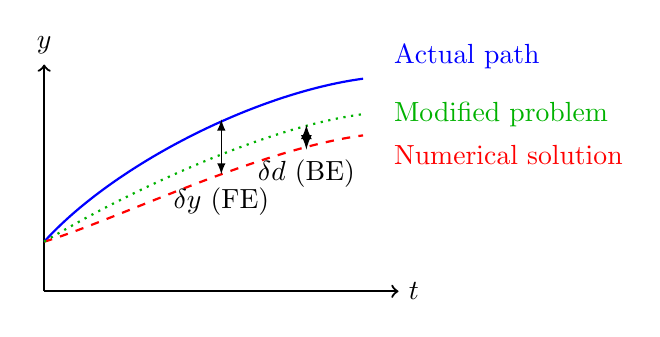
\begin{tikzpicture}[scale=0.9]
        % Axes
            \draw[->, thick] (0,0) -- (5,0) node[right] {$t$};
            \draw[->, thick] (0,0) -- (0,3.2) node[above] {$y$};

            % True trajectory (blue, smooth curve, higher)
            \draw[thick, blue] (0,0.7) .. controls (1,1.8) and (3,2.8) .. (4.5,3.0);
            \node[blue, above right] at (4.8,3.0) {Actual path};

            % Computed trajectory (red, dashed, lower and more curved)
            \draw[thick, red, dashed] (0,0.7) .. controls (1,1.0) and (3,2.0) .. (4.5,2.2);
            \node[red, below right] at (4.8,2.2) {Numerical solution};

            % Modified equation trajectory (green, dotted, between true and computed)
            \draw[thick, green!70!black, dotted] (0,0.7) .. controls (1,1.3) and (3,2.3) .. (4.5,2.5);
            \node[green!70!black, right] at (4.8,2.5) {Modified problem};

            % Forward error arrow: from computed to true (diagonal up)
            \draw[<->,>=latex] (2.5,1.65) -- (2.5,2.425);
            \node[below] at (2.5,1.6) {\(\delta y\) (FE)};

            % Backward error arrow: from computed to modified (vertical up)
            \draw[<->,>=latex, thick] (3.7,2) -- (3.7,2.35);
            \node[below] at (3.7,2) {\(\delta d\) (BE)};

    \end{tikzpicture}
    \caption{Backward error: the computed solution solves a slightly perturbed problem exactly—often closer than the forward error.}
    \label{fig:backward-error}
\end{figure}

\subsection{Controlling Error}
\label{sec:practical-strategies}

Effective error control follows a systematic approach:

\begin{enumerate}
    \item \textbf{Problem Reformulation:} Address ill-conditioning at the mathematical level
    \item \textbf{Method Selection:} Choose algorithms suited to problem characteristics
    \item \textbf{Adaptive Control:} Automatically adjust computational parameters
    \item \textbf{Post-processing:} Apply error reduction techniques
    \item \textbf{Verification:} Validate results through multiple approaches
\end{enumerate}

\begin{figure}[htbp]
    \centering
    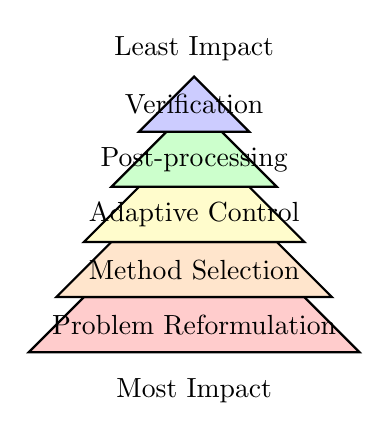
\begin{tikzpicture}[scale=0.7]
        % Error control pyramid
        \draw[thick, fill=red!20] (0,0) -- (6,0) -- (5,1) -- (1,1) -- cycle;
        \node at (3,0.5) {Problem Reformulation};

        \draw[thick, fill=orange!20] (0.5,1) -- (5.5,1) -- (4.5,2) -- (1.5,2) -- cycle;
        \node at (3,1.5) {Method Selection};

        \draw[thick, fill=yellow!20] (1,2) -- (5,2) -- (4,3) -- (2,3) -- cycle;
        \node at (3,2.5) {Adaptive Control};

        \draw[thick, fill=green!20] (1.5,3) -- (4.5,3) -- (3.5,4) -- (2.5,4) -- cycle;
        \node at (3,3.5) {Post-processing};

        \draw[thick, fill=blue!20] (2,4) -- (4,4) -- (3,5) -- cycle;
        \node at (3,4.5) {Verification};

        \node at (3,-0.7) {Most Impact};
        \node at (3,5.5) {Least Impact};
    \end{tikzpicture}
    \caption{Error control hierarchy: address fundamental issues first.}
    \label{fig:error-hierarchy}
\end{figure}

\subsection{Method Selection Guidelines}
\label{subsec:method-selection}

\begin{center}
    \begin{tabular}{@{}l l l@{}}
        \toprule
        \textbf{Problem}  & \textbf{Recommended Methods}          & \textbf{Considerations}        \\
        \midrule
        Smooth ODEs       & High-order Runge-Kutta, Adams methods & Efficiency over stability      \\
        Stiff ODEs        & Implicit methods (BDF, RADAU)         & $A$- or $L$-stability required \\
        Oscillatory       & Symplectic, exponential integrators   & Preserve energy/oscillations   \\
        Conservation laws & Geometric integrators                 & Structure preservation         \\
        Rough data        & Robust methods, regularization        & Stability over high order      \\
        \bottomrule
    \end{tabular}
\end{center}

\subsection{Algorithmic Best Practices}
\label{subsec:best-practices}

\paragraph{Numerical Hygiene}
\begin{itemize}
    \item Avoid subtracting nearly equal numbers
    \item Use stable algorithms (QR vs. normal equations)
    \item Scale problems to avoid extreme magnitudes
    \item Check intermediate results for sanity
\end{itemize}

\paragraph{Error Monitoring}
\begin{itemize}
    \item Track residuals and error estimates
    \item Use multiple precision levels for comparison
    \item Implement convergence tests with multiple criteria
    \item Monitor conservation quantities when applicable
\end{itemize}

\section{Case Studies in Error Analysis}
\label{sec:case-studies}

\subsection{Case Study 1: The Quadratic Formula}
\label{subsec:quadratic-case}

Consider solving $ax^2 + bx + c = 0$ with $a = 1$, $b = -2000$, $c = 1$.

\paragraph{Standard Formula (Poor):}
\[
    x = \frac{2000 \pm \sqrt{4000000 - 4}}{2} = \frac{2000 \pm 1999.999}{2}
\]
One root suffers catastrophic cancellation: $x_1 = \frac{2000 - 1999.999}{2} = 0.0005$

\paragraph{Improved Formula (Good):}
Use $x_1 x_2 = c/a = 1$, so:
\[
    x_1 = \frac{2c}{-b - \sqrt{b^2 - 4ac}} = \frac{2}{2000 + 1999.999} = \frac{1}{1999.9995}
\]

\subsection{Case Study 2: Computing \texorpdfstring{$e^x - 1$}{ex - 1} for Small \texorpdfstring{$x$}{x}}
\label{subsec:exp-case}

\paragraph{Direct Computation (Poor):}
For $x = 10^{-8}$: $e^x - 1 = 1.00000001 - 1 = 10^{-8}$ (loses digits)

\paragraph{Series Expansion (Good):}
\[
    e^x - 1 = x + \frac{x^2}{2!} + \frac{x^3}{3!} + \cdots
\]
For small $x$, truncate after a few terms.

\paragraph{Built-in Function (Best):}
Use \texttt{expm1(x)} which is designed for this purpose.

\section{Summary and Final Insights}
\label{sec:final-summary}

\begin{remark}[title=Fundamental Principles]{}{}
    \begin{enumerate}
        \item \textbf{Error is inevitable.} Every computation introduces approximation; the goal is to understand and control it.

        \item \textbf{Stability dominates accuracy.} A stable method with modest accuracy often outperforms an unstable high-order scheme.

        \item \textbf{Conditioning reveals problem difficulty.} Large condition numbers signal fundamental limitations, not implementation flaws.

        \item \textbf{Structure preservation matters.} For long-time integration, qualitative correctness can be more important than pointwise accuracy.

        \item \textbf{Multiple perspectives illuminate.} Forward, backward, and probabilistic error analyses each reveal different aspects of computational behavior.
    \end{enumerate}
\end{remark}

\subsection{The Error Analysis Toolkit}
\label{subsec:toolkit}

\begin{description}
    \item[Theoretical Tools] Condition numbers, stability analysis, convergence theory
    \item[Computational Tools] Adaptive methods, error estimation, residual monitoring
    \item[Diagnostic Tools] Multiple precision, alternative algorithms, conservation checks
    \item[Preventive Tools] Problem reformulation, method selection, numerical hygiene
\end{description}


\begin{remark}{Final Thought}{}
    \textbf{Error analysis is not just about finding mistakes—it's about understanding the fundamental limits and possibilities of computation.}

    Master these principles, and you'll develop an intuition for when numerical results can be trusted and when they require deeper investigation.
\end{remark}
